
\documentclass[ review  , 3p ]{elsarticle}
%default = preprint (single sapce), review = doublespace
%detail class option: https://www.elsevier.com/__data/assets/pdf_file/0008/56843/elsdoc-1.pdf

% eliminate "Preprinted to Elsevier"
\makeatletter
\def\ps@pprintTitle{%
 \let\@oddhead\@empty
 \let\@evenhead\@empty
 \def\@oddfoot{\centerline{\thepage}}%
 \let\@evenfoot\@oddfoot}
\makeatother

%%% Begin My package additions %%%%%%%%%%%%%%%%%%%
\usepackage[hyphens]{url}



\usepackage{lineno} % add
\providecommand{\tightlist}{%
  \setlength{\itemsep}{0pt}\setlength{\parskip}{0pt}}

\usepackage{graphicx}

\usepackage{zxjatype}
\usepackage{xeCJK}
\setCJKmainfont{ipaexm.ttf}
\setCJKsansfont{ipaexg.ttf}
\setCJKmonofont{ipaexg.ttf}

\usepackage{color}

\usepackage{booktabs}
\usepackage{longtable}
\usepackage{array}
\usepackage{multirow}
\usepackage{wrapfig}
\usepackage{float}
\usepackage{colortbl}
\usepackage{pdflscape}
\usepackage{tabu}
\usepackage{threeparttable}
\usepackage{threeparttablex}
\usepackage[normalem]{ulem}
\usepackage{makecell}
\usepackage{xcolor}


%\usepackage{xpatch}
%\xpatchcmd{\MaketitleBox}{\hrule}{}{}{}% remove first horizontal rule (above abstract)
%\xpatchcmd{\MaketitleBox}{\hrule}{}{}{}% remoce second horizonral rule (below keywords)
%%%%%%%%%%%%%%%% end my additions to header

\usepackage[T1]{fontenc}
\usepackage{lmodern}
\usepackage{amssymb,amsmath}
\usepackage{ifxetex,ifluatex}
\usepackage{fixltx2e} % provides \textsubscript
% use upquote if available, for straight quotes in verbatim environments
\IfFileExists{upquote.sty}{\usepackage{upquote}}{}
\ifnum 0\ifxetex 1\fi\ifluatex 1\fi=0 % if pdftex
  \usepackage[utf8]{inputenc}
\else % if luatex or xelatex
  \usepackage{fontspec}
  \ifxetex
    \usepackage{xltxtra,xunicode}
  \fi
  \defaultfontfeatures{Mapping=tex-text,Scale=MatchLowercase}
  \newcommand{\euro}{€}
\fi
% use microtype if available
\IfFileExists{microtype.sty}{\usepackage{microtype}}{}
\bibliographystyle{elsarticle-harvard}
\usepackage{tabularx}
\ifxetex
  \usepackage[setpagesize=false, % page size defined by xetex
              unicode=false, % unicode breaks when used with xetex
              xetex]{hyperref}
\else
  \usepackage[unicode=true]{hyperref}
\fi
\hypersetup{breaklinks=true,
            bookmarks=true,
            pdfauthor={},
            pdftitle={Short Paper},
            colorlinks=false,
            urlcolor=blue,
            linkcolor=magenta,
            pdfborder={0 0 0}}
\urlstyle{same}  % don't use monospace font for urls

\setcounter{secnumdepth}{5}

\newlength{\cslhangindent}
\setlength{\cslhangindent}{1.5em}
\newlength{\csllabelwidth}
\setlength{\csllabelwidth}{3em}
\newenvironment{CSLReferences}[3] % #1 hanging-ident, #2 entry spacing
 {% don't indent paragraphs
  \setlength{\parindent}{0pt}
  % turn on hanging indent if param 1 is 1
  \ifodd #1 \everypar{\setlength{\hangindent}{\cslhangindent}}\ignorespaces\fi
  % set entry spacing
  \ifnum #2 > 0
  \setlength{\parskip}{#2\baselineskip}
  \fi
 }%
 {}
\usepackage{calc} % for \widthof, \maxof
\newcommand{\CSLBlock}[1]{#1\hfill\break}
\newcommand{\CSLLeftMargin}[1]{\parbox[t]{\maxof{\widthof{#1}}{\csllabelwidth}}{#1}}
\newcommand{\CSLRightInline}[1]{\parbox[t]{\linewidth}{#1}}
\newcommand{\CSLIndent}[1]{\hspace{\cslhangindent}#1}

% Pandoc toggle for numbering sections (defaults to be off)


% Pandoc header


\begin{document}
  \begin{frontmatter}

    \title{Charitable Giving, Tax Reform, and Government Efficiency\tnoteref{1}}
            \tnotetext[1]{This research is base on}
                \author[Osaka University]{
      Hiroki Kato 
       \corref{*} }
     \ead{vge008kh@stundent.econ.osaka-u.ac.jp}   %to avoid auto-link, use \@ instead of @
        \author[Chiba University]{
      Tsuyoshi Goto 
      }
      %to avoid auto-link, use \@ instead of @
        \author[Kobe University]{
      Yong-Rok Kim 
      }
      %to avoid auto-link, use \@ instead of @
            \address[Osaka University]{Graduate School of Economics, Osaka University, Japan}
        \address[Chiba University]{Graduate School of Economics, Chiba University, Japan}
        \address[Kobe University]{Graduate School of Economics, Kobe University, Japan}
            \cortext[*]{Corresponding Author.}
      
        \begin{abstract}
      Brah
    \end{abstract}
      
        \begin{keyword}
      Charitable giving, Giving price, Tax reform, Governement efficiency, South Korea
       \JEL{D91, I10, I18} 
    \end{keyword}
    
  \end{frontmatter}

  \hypertarget{introduction}{%
  \section{Introduction}\label{introduction}}
  
  Placeholder
  
  \hypertarget{charitable-giving-and-taxiation}{%
  \subsection{Charitable Giving and Taxiation}\label{charitable-giving-and-taxiation}}
  
  \hypertarget{summary-in-short}{%
  \subsection{Summary in short}\label{summary-in-short}}
  
  \hypertarget{south-korean-tax-reform}{%
  \subsection{South Korean tax reform}\label{south-korean-tax-reform}}
  
  \hypertarget{related-literature}{%
  \subsection{Related Literature}\label{related-literature}}
  
  \hypertarget{research-about-tax-price-elasticity-of-charitable-donations}{%
  \subsection{Research about tax price elasticity of charitable donations}\label{research-about-tax-price-elasticity-of-charitable-donations}}
  
  \hypertarget{research-about-perception-towards-the-government-and-donationtax-payment.}{%
  \subsection{Research about perception towards the government and donation/tax payment.}\label{research-about-perception-towards-the-government-and-donationtax-payment.}}
  
  \hypertarget{why-political-trust}{%
  \subsection{Why Political Trust?}\label{why-political-trust}}
  
  \hypertarget{institutional-background}{%
  \section{Institutional background}\label{institutional-background}}
  
  Placeholder
  
  \hypertarget{tax-relief-for-charitable-giving-by-tax-deduction-and-tax-credit}{%
  \subsection{Tax relief for charitable giving by tax deduction and tax credit}\label{tax-relief-for-charitable-giving-by-tax-deduction-and-tax-credit}}
  
  \hypertarget{korean-tax-reform-in-2014-need-modification-by-kim-san}{%
  \subsection{Korean tax reform in 2014 (Need modification by Kim san)}\label{korean-tax-reform-in-2014-need-modification-by-kim-san}}
  
  \hypertarget{data}{%
  \section{Data}\label{data}}
  
  \hypertarget{national-survey-of-tax-and-benefit-nastab}{%
  \subsection{National Survey of Tax and Benefit (NaSTaB)}\label{national-survey-of-tax-and-benefit-nastab}}
  
  \begin{itemize}
  \tightlist
  \item
    The Korea Institute of Taxation and Finance implements the financial panel survey to study the tax burden of households and the benefits that households receive from goverment.
  \item
    The subjects of this survey are general household and household members living in 15 cities and provinces nationwide.
  \item
    This survey is based on a face-to-face interview. If it is difficult for investigators to meet subjects, another family member answers on behalf of him.
  \item
    Survey items: Annual taxable income (last year), charitable donations (last year), trust for politicians (5-Likert scale), and other covariates (age, education, gender etc.).
  \item
    Survey period: 2008 \textasciitilde{} 2019
  
    \begin{itemize}
    \tightlist
    \item
      We use survey data after 2013 to focus on tax policy change in 2014.
    \end{itemize}
  \end{itemize}
  
  \hypertarget{time-series-of-chariable-giving}{%
  \subsection{Time Series of Chariable Giving}\label{time-series-of-chariable-giving}}
  
  \begin{figure}
  
  {\centering 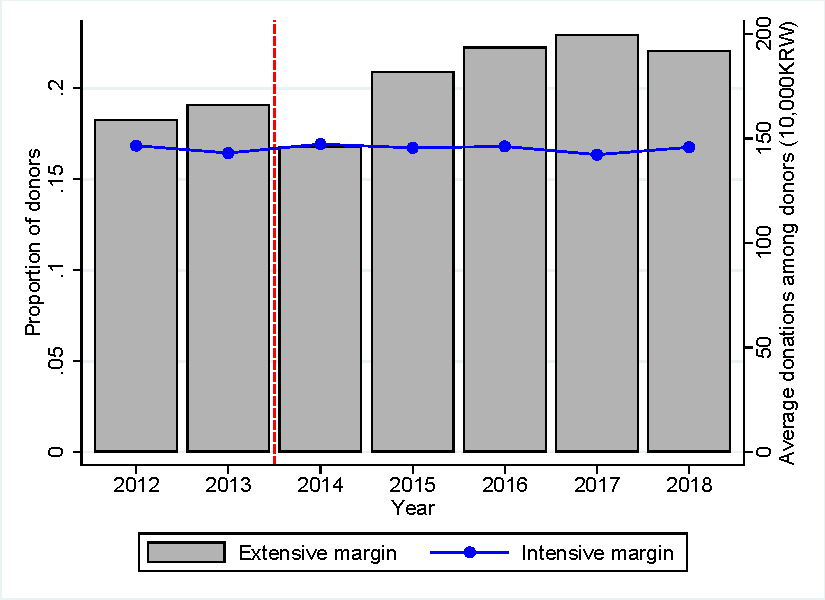
\includegraphics[width=0.9\linewidth]{C:/Users/vge00/Desktop/NaSTaB/_assets/SummaryOutcome} 
  
  }
  
  \caption{Proportion of Donors and Average Donations among Donors}\label{fig:unnamed-chunk-1}
  \end{figure}
  
  \hypertarget{summary-statistics}{%
  \subsection{Summary Statistics}\label{summary-statistics}}
  
  \begin{table}
  
  \caption{\label{tab:kableSummaryCovariate}Summary Statistics}
  \centering
  \fontsize{8}{10}\selectfont
  \begin{tabular}[t]{lcccccccc}
  \toprule
   & N & Mean & Std.Dev. & Min & p25 & p50 & p75 & Max\\
  \midrule
  \addlinespace[0.3em]
  \multicolumn{9}{l}{\textbf{Income and Giving Price}}\\
  \hspace{1em}Annual taxable income (unit: 10,000KRW) & 53269 & 1876.121 & 2700.965 & 0.00 & 0.00 & 900.00 & 2902.445 & 91772.00\\
  \hspace{1em}Giving Price & 62878 & 0.858 & 0.036 & 0.62 & 0.85 & 0.85 & 0.850 & 0.94\\
  \addlinespace[0.3em]
  \multicolumn{9}{l}{\textbf{Charitable Donations}}\\
  \hspace{1em}Annual charitable giving (unit: 10,000KRW) & 67849 & 29.522 & 132.914 & 0.00 & 0.00 & 0.00 & 0.000 & 10000.00\\
  \hspace{1em}dummy of Donation > 0 & 67849 & 0.203 & 0.402 & 0.00 & 0.00 & 0.00 & 0.000 & 1.00\\
  \addlinespace[0.3em]
  \multicolumn{9}{l}{\textbf{Government Efficiency}}\\
  \hspace{1em}Current Tax-Welfare Balance & 29272 & -0.137 & 0.889 & -2.00 & -1.00 & 0.00 & 0.000 & 2.00\\
  \hspace{1em}Ideal Tax-Welfare Balance & 29273 & 0.541 & 0.721 & -2.00 & 0.00 & 0.00 & 1.000 & 2.00\\
  \addlinespace[0.3em]
  \multicolumn{9}{l}{\textbf{Individual Characteristics}}\\
  \hspace{1em}Age & 67848 & 51.348 & 15.806 & 24.00 & 39.00 & 50.00 & 62.000 & 104.00\\
  \hspace{1em}Female dummy & 67848 & 0.525 & 0.499 & 0.00 & 0.00 & 1.00 & 1.000 & 1.00\\
  \hspace{1em}University graduate & 67842 & 0.411 & 0.492 & 0.00 & 0.00 & 0.00 & 1.000 & 1.00\\
  \hspace{1em}High school graduate & 67842 & 0.350 & 0.477 & 0.00 & 0.00 & 0.00 & 1.000 & 1.00\\
  \hspace{1em}Junior high school graduate & 67842 & 0.238 & 0.426 & 0.00 & 0.00 & 0.00 & 0.000 & 1.00\\
  \bottomrule
  \end{tabular}
  \end{table}
  
  \hypertarget{what-is-giving-price}{%
  \subsection{What is Giving Price?}\label{what-is-giving-price}}
  
  Consider allocation between private consumptions (\(x_i\)) and charitable giving (\(g_i\)).
  Let \(y_i\) be pre-tax total income.
  Then, the budget constraint is
  
  \[
      x_i + g_i = y_i - T_i(y_i, g_i),
  \]
  
  where \(T_i\) is tax amount depending on the pre-tax income and charitable giving.
  
  \hypertarget{determination-of-tax-amount}{%
  \subsection{Determination of Tax Amount}\label{determination-of-tax-amount}}
  
  Tax deduction reduces taxable income by giving, that is,
  
  \[
      T_i = \tau(y_i - g_i) \cdot (y_i - g_i),
  \]
  
  where \(\tau(\cdot)\) is the marginal income tax rate which is determined by \(y_i - g_i\).
  
  Tax credit reduces tax amount directly, that is,
  
  \[
      T_i = \tau(y_i)\cdot y_i - m g_i,
  \]
  
  where \(m \in [0, 1]\) is the tax credit rate.
  
  \hypertarget{derive-giving-price}{%
  \subsection{Derive Giving Price}\label{derive-giving-price}}
  
  Under the tax deduction system, the budget constraint is
  
  \[
      x_i + [1 - \tau(y_i - g_i)]g_i = [1 - \tau(y_i - g_i)] y_i.
  \]
  
  Thus, the giving price of tax deduction system is \(p_i^{d} = 1 - \tau(y_i - g_i)\).
  
  Under the tax credit system, the budget constraint is
  
  \[
      x_i + (1 - m) g_i = [1 - \tau(y_i)] y_i.
  \]
  
  Thus, the giving price of tax credit system is \(p_i^c = 1 - m\).
  
  \hypertarget{construct-giving-price}{%
  \subsection{Construct Giving Price}\label{construct-giving-price}}
  
  In the South Korea, the tax policy about charitable giving drastically changed in 2014.
  
  \begin{itemize}
  \tightlist
  \item
    tax deduction (before 2014): \(\text{Price}_i = 1 - \tau(y_i - g_i)\)
  
    \begin{itemize}
    \tightlist
    \item
      the giving price is endogenous because people can manipulate \(\tau(y_i - g_i)\) using the charitable giving \(g_i\). Since this problem is caused by \emph{last} donations, we use the giving price applying to the \emph{first} donations (\textbf{first price}). The first price is calculate by \(\tau(y_i)\) where \(y_i\) is the annual taxable income reported in the NaSTaB.
    \end{itemize}
  \item
    tax credit (after 2014): \(\text{Price}_i = 1 - m\)
  
    \begin{itemize}
    \tightlist
    \item
      In the South Korea, the tax credit rate determines exogeneity, \(m = 0.15\).
    \end{itemize}
  \end{itemize}
  
  \hypertarget{income-distribution-and-giving-price}{%
  \subsection{Income Distribution and Giving Price}\label{income-distribution-and-giving-price}}
  
  \begin{figure}
  
  {\centering 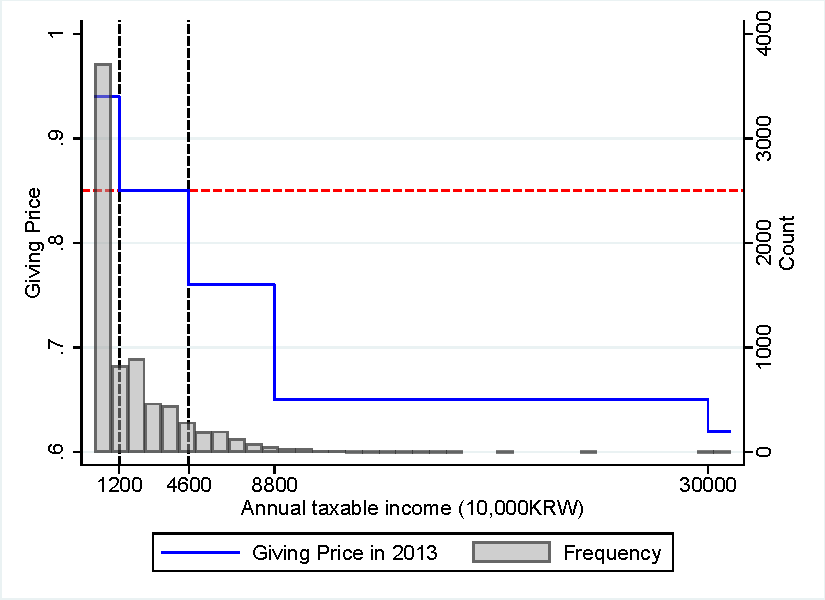
\includegraphics[width=0.9\linewidth]{C:/Users/vge00/Desktop/NaSTaB/_assets/SummaryPriceChange} 
  
  }
  
  \caption{Income Distribution and Giving Price in 2013}\label{fig:unnamed-chunk-2}
  \end{figure}
  
  \hypertarget{empirical-strategy}{%
  \subsection{Empirical Strategy}\label{empirical-strategy}}
  
  Our baseline regression equation is
  
  \[
      \log(\text{Giving}_{ijt}) = 
      \alpha_i + \beta_1 \log(\text{Price}_{ijt}) + \delta X_{ijt} + \lambda_t + \epsilon_{ijt}.
  \]
  
  \begin{itemize}
  \tightlist
  \item
    \(\log(\text{Giving}_{ijt})\) is logarithm of individual \(i\)'s charitable giving in year \(t\).
  \item
    \(\log(\text{Price}_{ijt})\) is logarithm of individual \(i\)'s giving price in year \(t\).
  \item
    \(\beta_1\) represents the price elasticity of giving.
  \item
    \(\alpha_i\) and \(\lambda_t\) are individual and time fixed effect, respectively.
  \end{itemize}
  
  \hypertarget{intensive-margin-and-extensive-margin}{%
  \subsection{Intensive Margin and Extensive Margin}\label{intensive-margin-and-extensive-margin}}
  
  Let \(D_{ijt}\) be a dummy variable taking 1 if individual \(i\) whose resident area \(j\) in year \(t\) donate in year \(t\)
  
  \begin{itemize}
  \tightlist
  \item
    Intensive margin: Estiamte \(\beta_1\) where outcome variable is \(\log(\text{Giving}_{ijt})\), using units with \(D_{ijt} = 1\).
  \item
    Extensive margin: Estimate \(\beta_1\) where outcome variable is \(D_{ijt}\).
  
    \begin{itemize}
    \tightlist
    \item
      Extensive-margin price elasticity can be calculated by \(\beta_1/\bar{D}\) where \(\bar{D}\) is the sample mean of \(D_{ijt}\).
    \end{itemize}
  \end{itemize}
  
  Covariates in each column corresponds to a column in a previous slide.
  
  \hypertarget{main-results}{%
  \section{Main Results}\label{main-results}}
  
  Placeholder
  
  \hypertarget{price-and-income-elasticity}{%
  \subsection{Price and Income Elasticity}\label{price-and-income-elasticity}}
  
  \hypertarget{baseline-regressions-result}{%
  \subsection{Baseline Regressions: Result}\label{baseline-regressions-result}}
  
  \hypertarget{intensive-margin-and-extensive-margin-result}{%
  \subsection{Intensive Margin and Extensive Margin: Result}\label{intensive-margin-and-extensive-margin-result}}
  
  \hypertarget{robustness-check}{%
  \subsection{Robustness Check}\label{robustness-check}}
  
  \hypertarget{robustness-check-1}{%
  \subsection{Robustness Check 1}\label{robustness-check-1}}
  
  \hypertarget{robustness-check-1-result}{%
  \subsection{Robustness Check 1: Result}\label{robustness-check-1-result}}
  
  \hypertarget{robustness-check-1-intensive-and-extensive-margin}{%
  \subsection{Robustness Check 1: Intensive and Extensive Margin}\label{robustness-check-1-intensive-and-extensive-margin}}
  
  \hypertarget{robust-check-2}{%
  \subsection{Robust Check 2}\label{robust-check-2}}
  
  \hypertarget{robustness-check-2-result}{%
  \subsection{Robustness Check 2: Result}\label{robustness-check-2-result}}
  
  \hypertarget{robustness-check-2-intensive-and-extensive-margin}{%
  \subsection{Robustness Check 2: Intensive and Extensive Margin}\label{robustness-check-2-intensive-and-extensive-margin}}
  
  \hypertarget{governement-efficient-and-price-elasticity}{%
  \section{Governement Efficient and Price Elasticity}\label{governement-efficient-and-price-elasticity}}
  
  Placeholder
  
  \hypertarget{government-efficiency}{%
  \subsection{Government Efficiency}\label{government-efficiency}}
  
  \hypertarget{construct-efficient-index}{%
  \subsection{Construct Efficient Index}\label{construct-efficient-index}}
  
  \hypertarget{histrogram-of-efficient-index}{%
  \subsection{Histrogram of Efficient Index}\label{histrogram-of-efficient-index}}
  
  \hypertarget{heterogenous-price-elasticity-by-governement-efficiency}{%
  \subsection{Heterogenous Price Elasticity by Governement Efficiency}\label{heterogenous-price-elasticity-by-governement-efficiency}}
  
  \hypertarget{efficient-groups-descriptive-stats}{%
  \subsection{Efficient Groups: Descriptive Stats}\label{efficient-groups-descriptive-stats}}
  
  \hypertarget{efficient-groups-descriptive-statis-extensive-margin}{%
  \subsection{Efficient Groups: Descriptive Statis (Extensive Margin)}\label{efficient-groups-descriptive-statis-extensive-margin}}
  
  \hypertarget{efficient-groups-descriptive-stats-intensive-margin}{%
  \subsection{Efficient Groups: Descriptive Stats (Intensive Margin)}\label{efficient-groups-descriptive-stats-intensive-margin}}
  
  \hypertarget{efficient-groups-estimation-results}{%
  \subsection{Efficient Groups: Estimation Results}\label{efficient-groups-estimation-results}}
  
  \hypertarget{robustness-check-2}{%
  \subsection{Robustness Check}\label{robustness-check-2}}
  
  \hypertarget{robustness-check-1-1}{%
  \subsection{Robustness Check 1}\label{robustness-check-1-1}}
  
  \hypertarget{robustness-check-1-estimation-results}{%
  \subsection{Robustness Check 1: Estimation Results}\label{robustness-check-1-estimation-results}}
  
  \hypertarget{robustness-check-2-1}{%
  \subsection{Robustness Check 2}\label{robustness-check-2-1}}
  
  \hypertarget{robustness-check-2-result-1}{%
  \subsection{Robustness Check 2: Result}\label{robustness-check-2-result-1}}
  
  \hypertarget{robustness-check-2-result-extensive-margin}{%
  \subsection{Robustness Check 2: Result (Extensive Margin)}\label{robustness-check-2-result-extensive-margin}}
  
  \hypertarget{robustness-check-2-result-intensive-margin}{%
  \subsection{Robustness Check 2: Result (Intensive Margin)}\label{robustness-check-2-result-intensive-margin}}
  
  \hypertarget{conclusions}{%
  \section{Conclusions}\label{conclusions}}
  
  \hypertarget{conclusions-1}{%
  \subsection{Conclusions}\label{conclusions-1}}
  
  \clearpage
  
  \hypertarget{references}{%
  \subsection*{References}\label{references}}
  \addcontentsline{toc}{subsection}{References}

\end{document}


